\documentclass[24pt,pdf,hyperref={unicode}]{beamer}
\usepackage[utf8]{inputenc}
\usepackage{aiml}

\begin{document}


\section{Задача регрессии}

\begin{frame}\frametitle{Манипулятор}
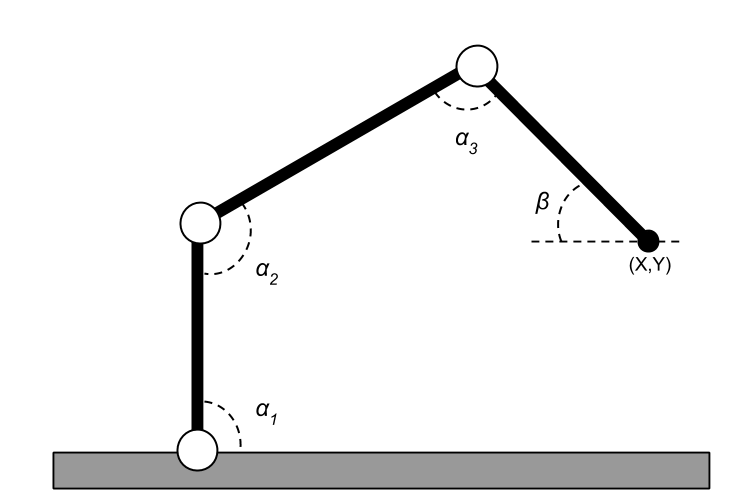
\includegraphics[width=\textwidth]{Images/Manipulator.png}
\end{frame}

\begin{frame}\frametitle{Манипулятор}
\begin{columns}[top]
\column{0.5\textwidth}
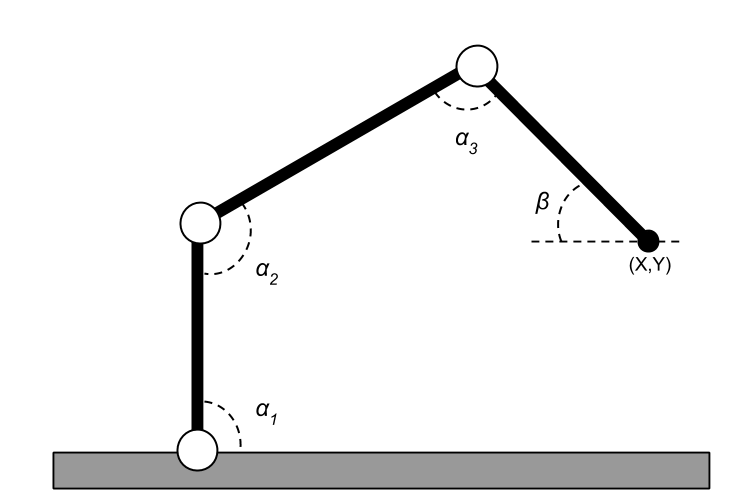
\includegraphics[width=\textwidth]{Images/Manipulator.png}
\column{0.5\textwidth}
\begin{center}
\begin{tikzpicture}[y=-1cm]
\node (input) at (0,0) {$(x,y,\beta)$};

\uncover<2->{
\node[rectangle,draw=black] (driver) at (0,1) {Driver};
\draw[->] (input)--(driver);
}

\uncover<3->{
\node (result) at (0,2) {\only<3-5>{$(\alpha_1,\alpha_2,\alpha_3)$}\only<6->{$(\alpha'_1,\alpha'_2,\alpha'_3)$}};
\draw[->] (driver)--(result);
}

\uncover<4->{
\node[rectangle,draw=black] (robot) at (0,3) {Robot};
\draw[->] (result)--(robot);
}

\uncover<5->{
\node (output) at (0,4) {$(x',y',\beta')$};
\draw[->] (robot)--(output);
}
\end{tikzpicture}
\end{center}
\uncover<6->{$$
(\alpha'_1,\alpha'_2,\alpha'_3)\overset{Robot}{\longrightarrow}(x',y',\beta')
$$}
\uncover<7->{$$
(\alpha_1,\alpha_2,\alpha_3)\overset{Robot}{\longrightarrow}(x,y,\beta)
$$}
\uncover<8->{$$
(x,y,\beta)\overset{?}{\longrightarrow}(\alpha_1,\alpha_2,\alpha_3)
$$}
\end{columns}
\end{frame}


\begin{frame}[t]\frametitle{Нейронные сети для юстировки манипулятора}
\begin{columns}[T]
\column{0.5\textwidth}
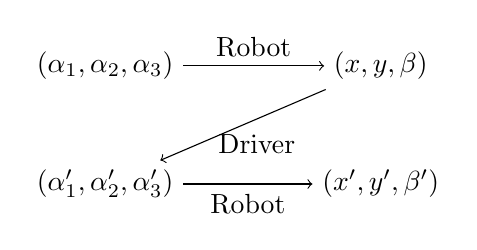
\begin{tikzpicture}[x=3.5cm,y=1.5cm]
\node (a1) at (0,0) {$(\alpha'_1,\alpha'_2,\alpha'_3)$};
\node (x1) at (1,0) {$(x',y',\beta')$};
\node (a0) at (0,1) {$(\alpha_1,\alpha_2,\alpha_3)$};
\node (x0) at (1,1) {$(x,y,\beta)$};
\path (a0) edge[->] node[above]{Robot} (x0);
\path (a1) edge[->] node[below]{Robot} (x1);
\path (x0) edge[->] node[below]{$\ \ \ $Driver} (a1);
\end{tikzpicture}
\smallskip
$$
\begin{array}{r c l}
\uncover<2->{(x,y,\beta) & \overset{Naive}{\longrightarrow} & (\alpha_1,\alpha_2,\alpha_3)} \\[0.2cm]
\uncover<4->{(\alpha'_1,\alpha'_2,\alpha'_3) & \overset{SubA}{\longrightarrow} & (\alpha_1,\alpha_2,\alpha_3)} \\[0.2cm]
\uncover<6->{(x',y',\beta') & \overset{SubX}{\longrightarrow} & (x,y,\beta)} \\[0.2cm]
\uncover<9->{(x,y,\beta) & \overset{Delta}{\longrightarrow} & (\alpha_1,\alpha_2,\alpha_3)-} \\
\uncover<9->{ & & -(\alpha'_1,\alpha'_2,\alpha'_3)} \\
\end{array}
$$




\column{0.5\textwidth}
\only<3>{
\begin{center}
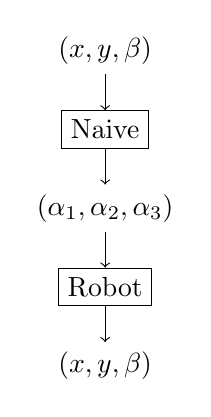
\begin{tikzpicture}[y=-1cm]
\node (input) at (0,0) {$(x,y,\beta)$};
\node[rectangle,draw=black] (driver) at (0,1) {Naive};
\draw[->] (input)--(driver);
\node (result) at (0,2) {$(\alpha_1,\alpha_2,\alpha_3)$};
\draw[->] (driver)--(result);
\node[rectangle,draw=black] (robot) at (0,3) {Robot};
\draw[->] (result)--(robot);
\node (output) at (0,4) {$(x,y,\beta)$};
\draw[->] (robot)--(output);
\end{tikzpicture}
\end{center}
}
\only<5>{
\begin{center}
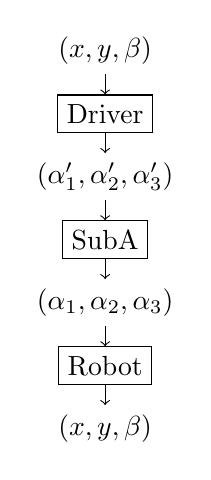
\begin{tikzpicture}[y=-0.8cm]
\node (input) at (0,0) {$(x,y,\beta)$};
\node[rectangle,draw=black] (driver) at (0,1) {Driver};
\draw[->] (input)--(driver);
\node (result) at (0,2) {$(\alpha'_1,\alpha'_2,\alpha'_3)$};
\draw[->] (driver)--(result);

\node[rectangle,draw=black] (neuro) at (0,3) {SubA};
\draw[->] (result)--(neuro);
\node (corrected) at (0,4) {$(\alpha_1,\alpha_2,\alpha_3)$};
\draw[->] (neuro)--(corrected);

\node[rectangle,draw=black] (robot) at (0,5) {Robot};
\draw[->] (corrected)--(robot);
\node (output) at (0,6) {$(x,y,\beta)$};
\draw[->] (robot)--(output);
\end{tikzpicture}
\end{center}
}
\only<7>{
\begin{center}
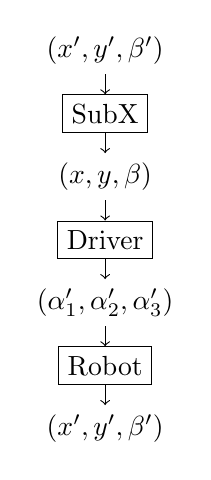
\begin{tikzpicture}[y=-0.8cm]
\node (input) at (0,0) {$(x',y',\beta')$};
\node[rectangle,draw=black] (neuro) at (0,1) {SubX};
\draw[->] (input)--(neuro);
\node (corrected) at (0,2) {$(x,y,\beta)$};
\draw[->] (neuro)--(corrected);
\node[rectangle,draw=black] (driver) at (0,3) {Driver};
\draw[->] (corrected)--(driver);
\node (result) at (0,4) {$(\alpha'_1,\alpha'_2,\alpha'_3)$};
\draw[->] (driver)--(result);
\node[rectangle,draw=black] (robot) at (0,5) {Robot};
\draw[->] (result)--(robot);
\node (output) at (0,6) {$(x',y',\beta')$};
\draw[->] (robot)--(output);
\end{tikzpicture}
\end{center}
}
\only<8>{
\begin{center}
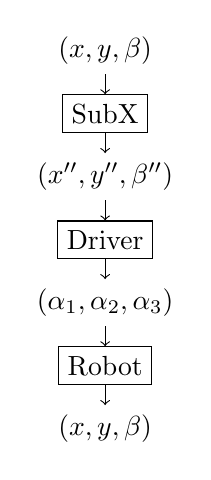
\begin{tikzpicture}[y=-0.8cm]
\node (input) at (0,0) {$(x,y,\beta)$};
\node[rectangle,draw=black] (neuro) at (0,1) {SubX};
\draw[->] (input)--(neuro);
\node (corrected) at (0,2) {$(x'',y'',\beta'')$};
\draw[->] (neuro)--(corrected);
\node[rectangle,draw=black] (driver) at (0,3) {Driver};
\draw[->] (corrected)--(driver);
\node (result) at (0,4) {$(\alpha_1,\alpha_2,\alpha_3)$};
\draw[->] (driver)--(result);
\node[rectangle,draw=black] (robot) at (0,5) {Robot};
\draw[->] (result)--(robot);
\node (output) at (0,6) {$(x,y,\beta)$};
\draw[->] (robot)--(output);
\end{tikzpicture}
\end{center}
}
\only<10>{
\begin{center}
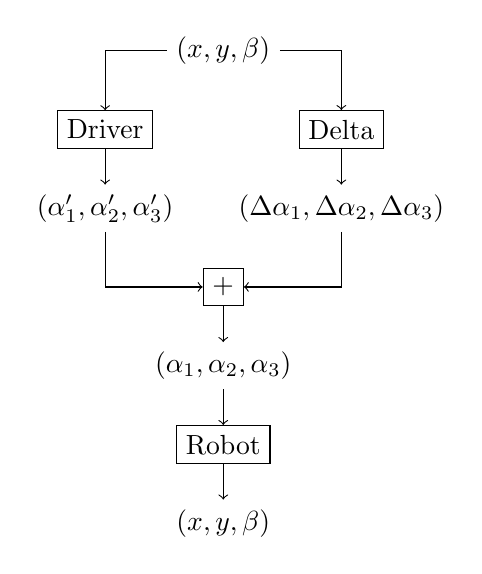
\begin{tikzpicture}[x=1.5cm,y=-1cm]
\node (input) at (0,0) {$(x,y,\beta)$};
\node[rectangle,draw=black] (driver) at (-1,1) {Driver};
\draw[->] (input) -| (driver);
\node (result) at (-1,2) {$(\alpha'_1,\alpha'_2,\alpha'_3)$};
\draw[->] (driver)--(result);

\node[rectangle,draw=black] (neuro) at (1,1) {Delta};
\draw[->] (input) -| (neuro);
\node (delta) at (1,2) {$(\Delta\alpha_1,\Delta\alpha_2,\Delta\alpha_3)$};
\draw[->] (neuro)--(delta);

\node[rectangle,draw=black] (plus) at (0,3) {$+$};
\draw[->] (delta) |- (plus);
\draw[->] (result) |- (plus);

\node (corrected) at (0,4) {$(\alpha_1,\alpha_2,\alpha_3)$};
\draw[->] (plus) -- (corrected);

\node[rectangle,draw=black] (robot) at (0,5) {Robot};
\draw[->] (corrected)--(robot);
\node (output) at (0,6) {$(x,y,\beta)$};
\draw[->] (robot)--(output);
\end{tikzpicture}
\end{center}
}

\end{columns}
\end{frame}

\end{document}